%!TEX root = report.tex

The final assignment used the code from the second assignment as basis, but a different dataset. The CIFAR-10 dataset was used, a dataset with 10 distinct classes such as airplane, dog or frog.

\subsection*{Input}
A different dataset meant that the format of the images also was different. The previous MNIST dataset used gray scale images which are 28 by 28 digits, while the CIFAR-10 dataset used colour images which are 32 by 32 pixels. 

Therefore the data first had to be reshaped in order to be able to be parsed by the neural network. The size of the filter also had to be changed, as well as the kernel sizes had to be increased from 4x4 to 5x5.

The dataset was split into six batches, five training batches and one test batch. For ease of use is the fifth training batch used as validation set, giving us a balanced training/validation/test set.

\subsection*{Architecture}
A number of settings for the convolutional neural network were tested in order to see which architecture gave the best scores. The size of nodes per hidden layers, the amount of hidden layers and amount of kernels were varied in order to see which gave the best result.

One of the issues we came across was a problem of overfitting. One of the methods to reduce overfitting available is to use dropout \cite{krizhevsky2012imagenet}\cite{srivastava2014dropout} .
 For each hidden layer used, a random mask of ones and zeroes is made and multiplied with the output of the layer. This randomly disables nodes while training in a hidden layer, essentially thinning the network temporarily by preventing those nodes into having incoming or outgoing connections.

Increasing the amount of kernels generally did not improve the results significantly, while increasing the runtime. Increasing the amount of nodes decreased the error percentages, up to a point. A too large network quickly became too complex and resulted in bad scores and long runtimes. Implementing the dropout method allowed the convolutional neural network to go from a test error of around 50\% to 33\%, which is quite an increase.

The results obtained and that are shown are using two almost equal architectures. The main difference between the two is that one uses local contrast normalization, while the other does not.

The architecture is as follows: first the image goes into the first convolution layer with 32 kernels, where the image is filtered and reduced from 32 by 32 to 14 by 14. The second convolution layer has 64 kernels and reduces the image size even further to a shape of 5 by 5. 

This is flattened and then sent to the first hidden layer with rectified linear units. This has 1600 inputs and reduces the data to 1250 outputs. The second hidden layer also uses rectified linear units and reduces the data further, from 1250 inputs to 128 outputs. 

Finally the output layer consists of logistic regression, which has ten potential outputs for each of the classes.

\subsection*{Results}
The results are presented in a graph, showing the change in the training, validation and test error over the epochs. Furthermore is there a graph with all of the kernels visualized. The results from two full runs are shown, one with local contrast normalization and one without. This allows us to also compare the effects of having local contrast normalization.

\begin{figure}[ht!]
	\centering
\begin{subfigure}[b]{0.45\textwidth}
	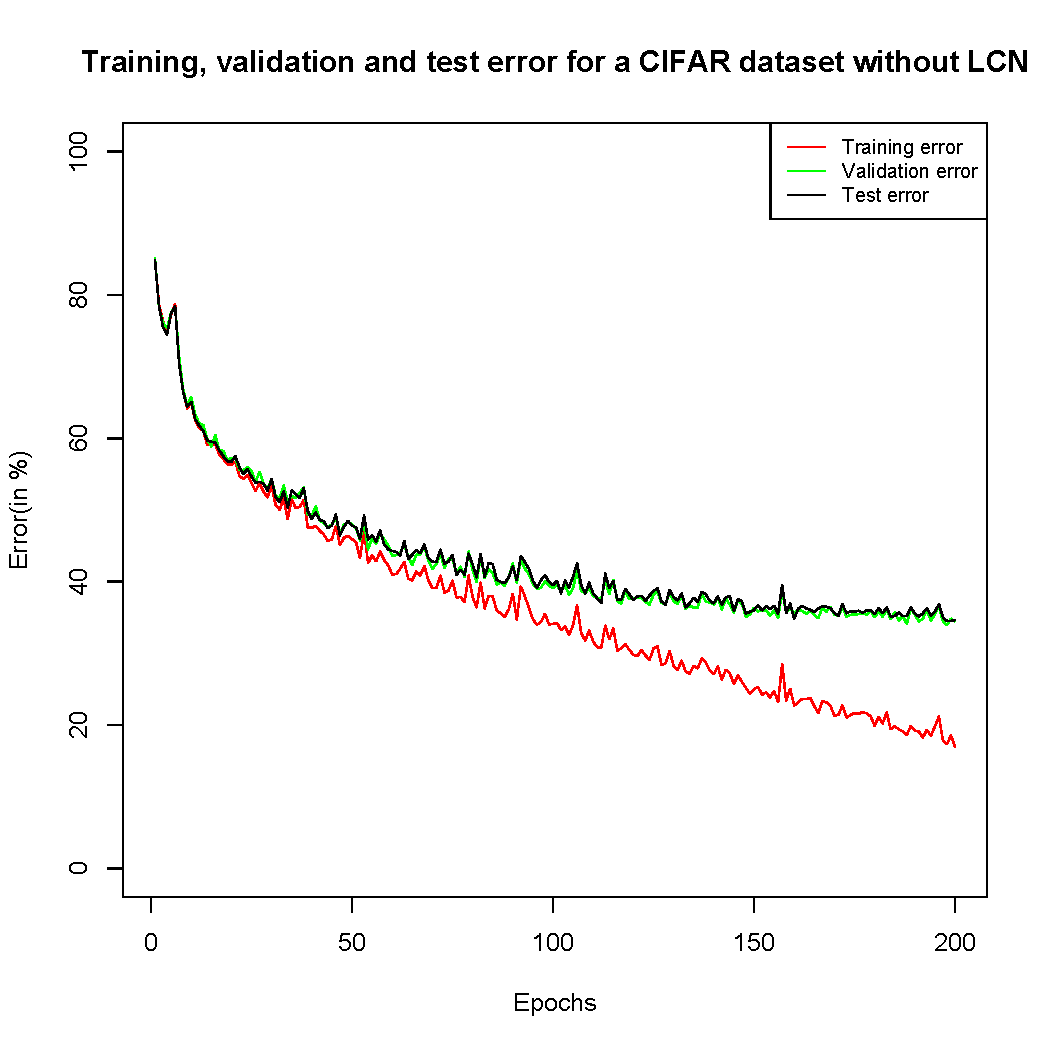
\includegraphics[width=\textwidth]{./img/Exercise3/Run1/errorplots.pdf}	
	\caption{The training, validation and test errors for a run over the number of epochs ran.}
	\label{fig:5:errorsNoLCN}
\end{subfigure}
\begin{subfigure}[b]{0.45\textwidth}
	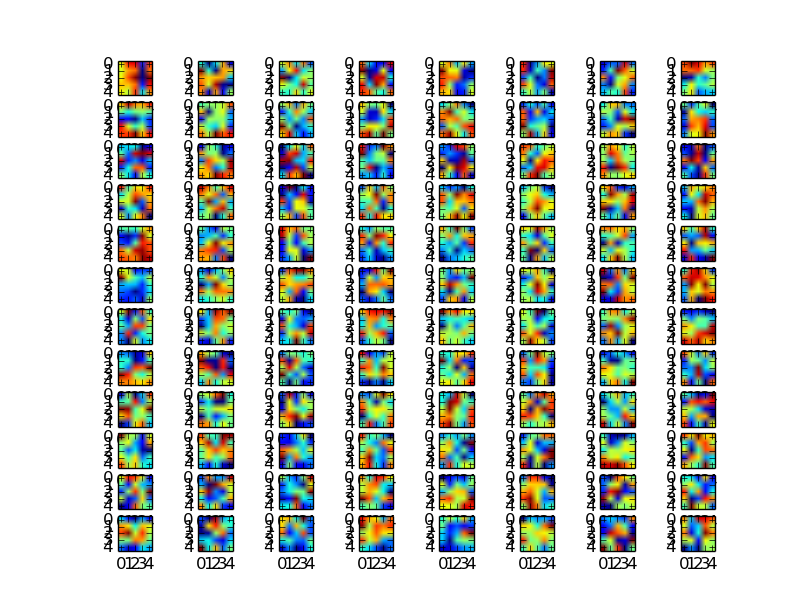
\includegraphics[width=\textwidth]{./img/Exercise3/Run1/3264end.png}	
	\caption{The resulting kernels for a run.}
	\label{fig:3:kernelsNoLCN}
\end{subfigure}
\caption{The results for a run without local contrast normalization.}
\end{figure}

The figures \ref{fig:3:kernelsNoLCN} and \ref{fig:4:kernelsLCN} show the kernels when using and abstaining from using local contrast normalization. As can be seen, there doesn't appear to be a large difference in the results.


\begin{figure}[ht!]
	\centering
\begin{subfigure}[b]{0.45\textwidth}
	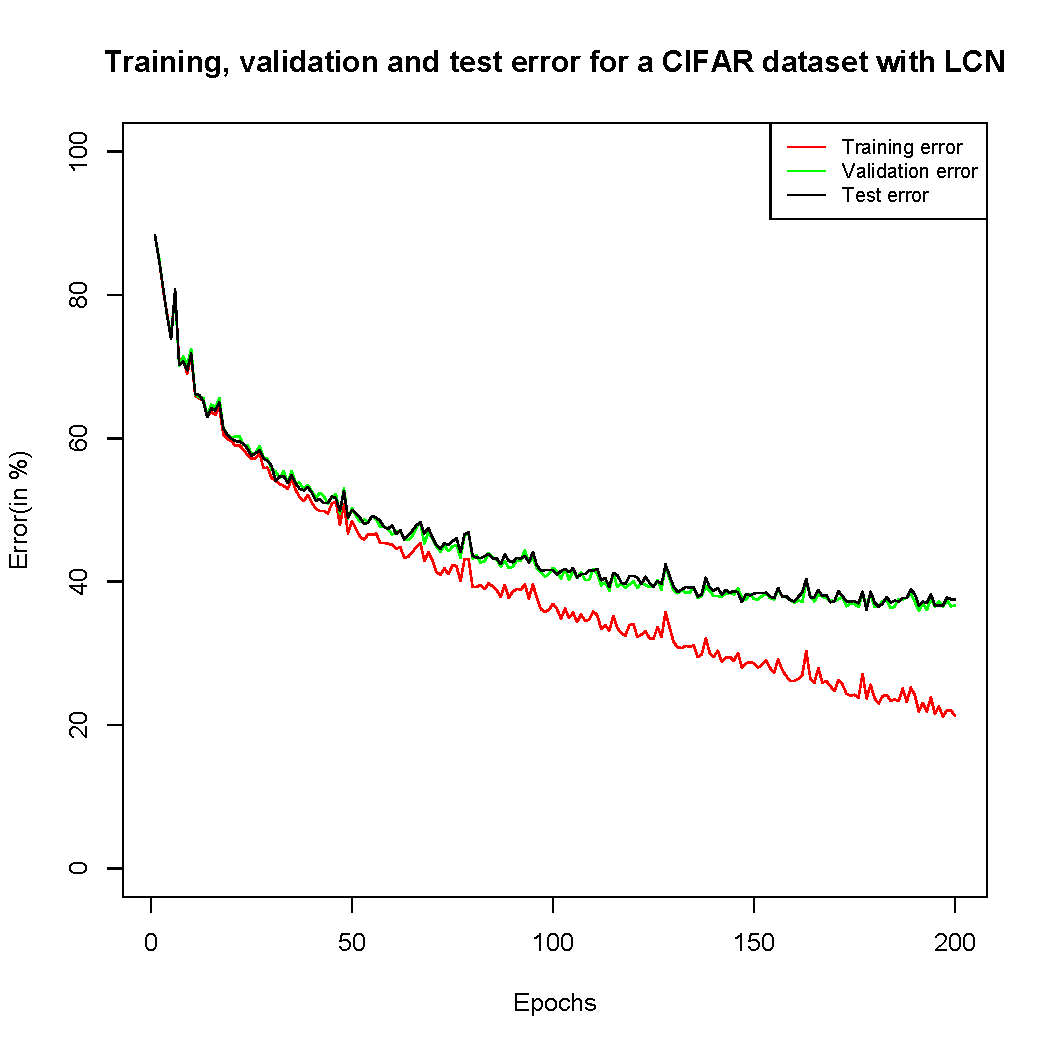
\includegraphics[width=\textwidth]{./img/Exercise3/Run2LCN/errorplots.pdf}	
	\caption{The training, validation and test errors for a run over the number of epochs ran.}
	\label{fig:6:errorsLCN}
\end{subfigure}
\begin{subfigure}[b]{0.45\textwidth}
	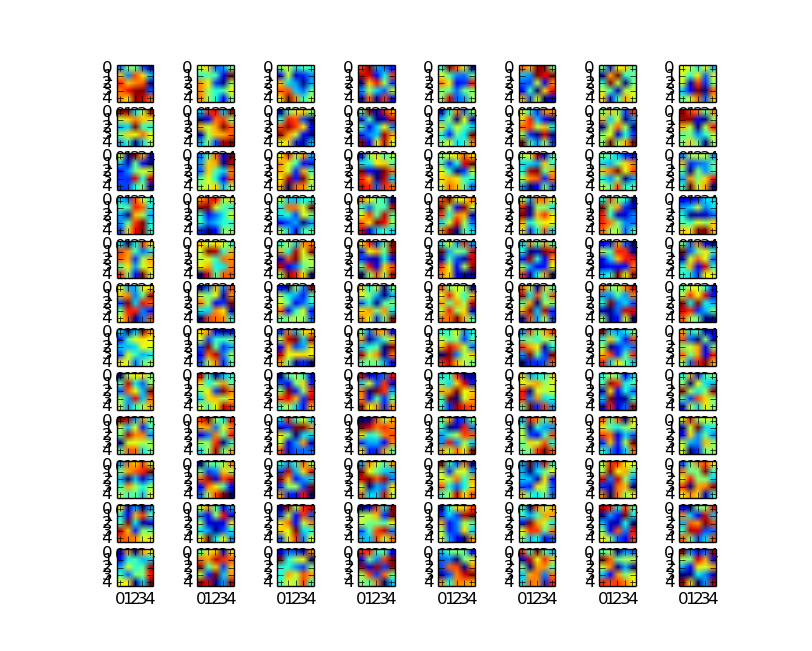
\includegraphics[width=\textwidth]{./img/Exercise3/Run2LCN/ass3final.png}	
	\caption{The resulting kernels for a run.}
	\label{fig:4:kernelsLCN}
\end{subfigure}
\caption{The results for a run with local contrast normalization.}
\end{figure}

This insignificant difference for using local contrast normalization also appears when looking at the difference in errors. Not using local contract normalization even gave us a better training error with about the same validation and test errors. 

The largest difference however, was the training time the algorithm needed to learn. Not using local contrast normalization took the system 34.13 minutes to learn and run 200 epochs, while if we were using local contrast normalization, the system took 201.16 minutes. Occam's razer dictates that the simpler model for the same results is better, and if you factor in learning time, then the best approach would be to not use local contrast normalization, even though it should have a positive effect on our results.

So this unfortunately begs the question whether our implementation of the learning curve optimalization was correct. Exercise 2 showed kernels with were in line with the expectated kernels when using learning curve optimalization, and those were reused for the third assignment, yet the kernels appear to not really differ between the runs with and without local contrast optimalization.

Nevertheless are the results good. A good architecture for the convolutional neural network on the CIFAR-10 dataset was able to get an 18\% test error according to the site where the CIFAR-10 dataset is located. With a fairly simple architecture and a non-optimized network due to time constraints, as well as missing performance boosting methods such as momentum, were we able to get a result of 32\%.
